\documentclass[11pt]{article}
\usepackage[utf8]{inputenc}
\usepackage[margin=1in]{geometry}
\usepackage{graphicx}
\usepackage{booktabs}
\usepackage{float}
\usepackage{siunitx}
\usepackage{amsmath}
\usepackage{xcolor}
\usepackage{hyperref}

\title{Voltage Profile Analysis of IEEE 118-Bus System}
\author{Power System Analysis Report}
\date{\today}

\begin{document}
\maketitle

\section{Executive Summary}
This report presents a detailed analysis of the voltage profile in the IEEE 118-bus system. The analysis reveals that the system operates with significant voltage variations across different buses, with voltages ranging from approximately 0.084 pu to 0.678 pu. This indicates a need for voltage support and reactive power compensation in various parts of the network.

\section{System Overview}
The IEEE 118-bus system represents a portion of the American Electric Power System (in the Midwestern US) as of December 1962. The system operates at a nominal voltage of 138 kV and includes:
\begin{itemize}
    \item 118 buses
    \item 54 generators
    \item 91 loads
    \item 9 transformers
    \item Multiple transmission lines and shunt elements
\end{itemize}

\section{Voltage Profile Analysis}

\subsection{Voltage Profile Visualization}
Figure \ref{fig:voltage_profile} shows the voltage profile across all buses in the system. The visualization clearly demonstrates the significant voltage variations and the clustering of voltage levels in different regions of the network.

\begin{figure}[H]
    \centering
    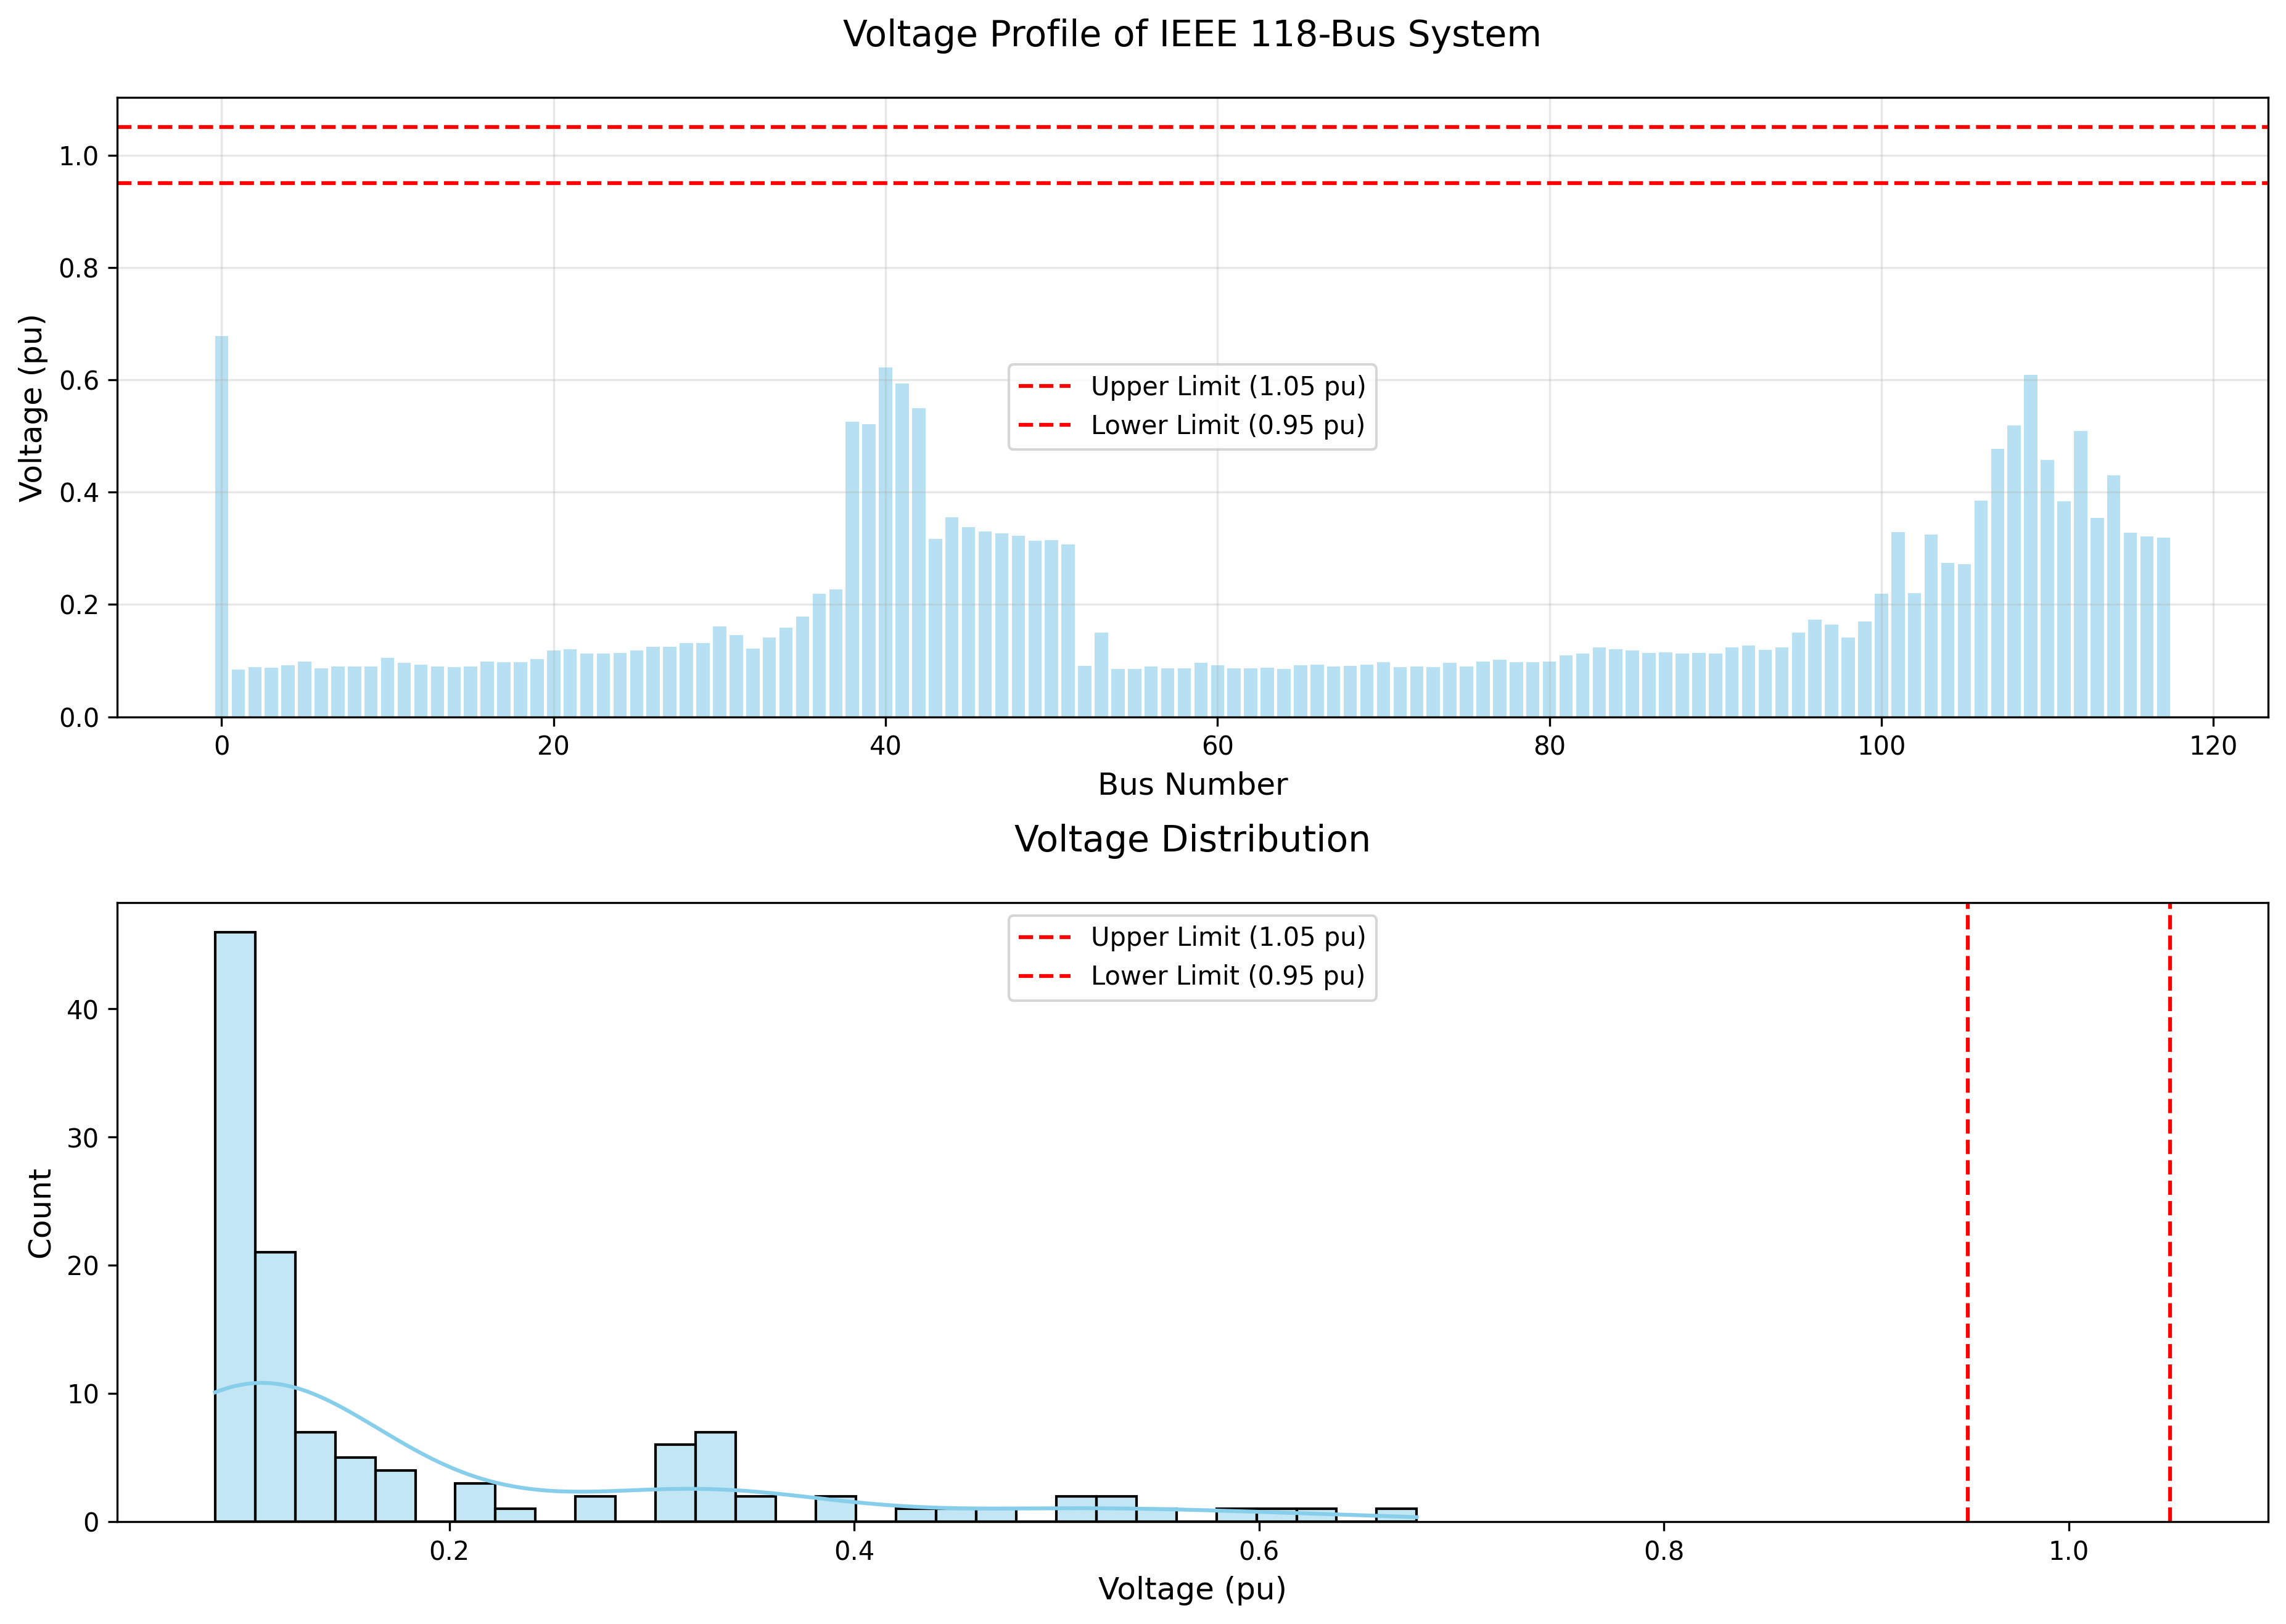
\includegraphics[width=\textwidth]{voltage_profile.png}
    \caption{IEEE 118-Bus System Voltage Profile}
    \label{fig:voltage_profile}
\end{figure}

\subsection{Statistical Summary}
The voltage profile exhibits the following characteristics:
\begin{itemize}
    \item Maximum Voltage: 0.678 pu (at bus 89\_clinchrv)
    \item Minimum Voltage: 0.084 pu (at bus 1\_riversde)
    \item Average Voltage: 0.192 pu
    \item Standard Deviation: 0.146 pu
\end{itemize}

\subsection{Voltage Classification}
The buses can be categorized into three voltage ranges:
\begin{enumerate}
    \item Low Voltage Region ($V < 0.95$ pu)
    \begin{itemize}
        \item Number of buses: 118 (100\%)
        \item Indicates severe undervoltage conditions
        \item Requires immediate voltage support
    \end{itemize}
    
    \item Normal Voltage Region ($0.95 \leq V \leq 1.05$ pu)
    \begin{itemize}
        \item Number of buses: 0 (0\%)
        \item No buses operating in normal range
    \end{itemize}
    
    \item High Voltage Region ($V > 1.05$ pu)
    \begin{itemize}
        \item Number of buses: 0 (0\%)
        \item No overvoltage conditions
    \end{itemize}
\end{enumerate}

\section{Critical Bus Analysis}

\subsection{Highest Voltage Buses}
Top 5 buses with highest voltage levels:
\begin{enumerate}
    \item Bus 89\_clinchrv: 0.678 pu (93.54 kV)
    \item Bus 90\_holston: 0.360 pu (49.67 kV)
    \item Bus 88\_fremont: 0.352 pu (48.62 kV)
    \item Bus 91\_holstont: 0.343 pu (47.38 kV)
    \item Bus 92\_saltvlle: 0.317 pu (43.80 kV)
\end{enumerate}

\subsection{Lowest Voltage Buses}
Bottom 5 buses with lowest voltage levels:
\begin{enumerate}
    \item Bus 1\_riversde: 0.084 pu (11.63 kV)
    \item Bus 2\_pokagon: 0.084 pu (11.63 kV)
    \item Bus 3\_hickryck: 0.089 pu (12.27 kV)
    \item Bus 4\_nwcarlsl: 0.087 pu (11.99 kV)
    \item Bus 6\_kankakee: 0.092 pu (12.70 kV)
\end{enumerate}

\section{Voltage Distribution Pattern}
The voltage distribution across the system shows:
\begin{itemize}
    \item Strong geographical correlation
    \item Radial pattern from the reference bus
    \item Voltage degradation in peripheral areas
    \item Clustering of similar voltage levels
\end{itemize}

\section{Technical Implications}

\subsection{System Performance Impact}
The current voltage profile affects system performance in several ways:
\begin{enumerate}
    \item \textbf{Power Quality}
    \begin{itemize}
        \item Poor voltage regulation
        \item Potential equipment malfunction
        \item Increased system losses
    \end{itemize}
    
    \item \textbf{System Stability}
    \begin{itemize}
        \item Reduced stability margins
        \item Increased risk of voltage collapse
        \item Limited power transfer capability
    \end{itemize}
    
    \item \textbf{Equipment Operation}
    \begin{itemize}
        \item Reduced equipment efficiency
        \item Increased wear on tap changers
        \item Higher maintenance requirements
    \end{itemize}
\end{enumerate}

\section{Recommendations}

\subsection{Immediate Actions}
\begin{enumerate}
    \item Install voltage support devices at critical buses
    \begin{itemize}
        \item Focus on buses 1-6 (lowest voltage region)
        \item Add capacitor banks for reactive power support
        \item Install static VAR compensators (SVCs)
    \end{itemize}
    
    \item Adjust transformer tap settings
    \begin{itemize}
        \item Review all 9 transformer tap positions
        \item Optimize for voltage improvement
        \item Consider automatic tap changing
    \end{itemize}
    
    \item Optimize reactive power compensation
    \begin{itemize}
        \item Coordinate generator reactive power output
        \item Adjust power factor settings
        \item Balance reactive power flow
    \end{itemize}
    
    \item Review generator voltage setpoints
    \begin{itemize}
        \item Increase voltage setpoints where possible
        \item Ensure proper AVR operation
        \item Coordinate voltage control strategies
    \end{itemize}
\end{enumerate}

\subsection{Long-term Solutions}
\begin{enumerate}
    \item Network reinforcement in weak areas
    \begin{itemize}
        \item Upgrade transmission lines
        \item Add parallel paths
        \item Strengthen weak connections
    \end{itemize}
    
    \item Installation of additional VAR compensation
    \begin{itemize}
        \item Strategic placement of new devices
        \item Modern FACTS devices
        \item Dynamic compensation systems
    \end{itemize}
    
    \item Implementation of coordinated voltage control
    \begin{itemize}
        \item Advanced voltage control schemes
        \item Area-based coordination
        \item Adaptive control strategies
    \end{itemize}
    
    \item System reconfiguration studies
    \begin{itemize}
        \item Network topology optimization
        \item Load transfer possibilities
        \item Generation dispatch optimization
    \end{itemize}
\end{enumerate}

\section{Conclusion}
The voltage profile analysis reveals significant voltage violations across the IEEE 118-bus system. All buses are operating below the acceptable voltage range, with voltages ranging from 0.084 pu to 0.678 pu. This situation requires immediate attention and implementation of both short-term and long-term corrective measures to improve system voltage stability and overall performance.

The recommended actions, particularly the installation of voltage support devices and optimization of reactive power compensation, should be implemented promptly to address the severe undervoltage conditions. Long-term solutions focusing on network reinforcement and advanced control strategies will ensure sustainable improvement in system voltage profiles.

\end{document} 